\documentclass[12pt,letterpaper]{article}

\usepackage[utf8]{inputenc}
\usepackage[T1]{fontenc}
\usepackage[spanish]{babel}
\usepackage{geometry}\geometry{margin=2.5cm}
\usepackage{amsmath}
\usepackage{amssymb}
\usepackage{graphicx}
\usepackage{booktabs}
\usepackage{float}
\usepackage{caption}
\usepackage{subcaption}
\usepackage{xcolor}
\usepackage{hyperref}
\usepackage{multirow}
\usepackage{array}
\usepackage{parskip}
\usepackage{fancyhdr}
\usepackage{siunitx}

\setlength{\headheight}{15pt}
\pagestyle{fancy}
\fancyhf{}
\rhead{Redes Inalámbricas Eficientes en Energía}
\lhead{Red LoRa Raw Solar — CU Stadium}
\cfoot{\thepage}

\definecolor{green3}{RGB}{56,142,60}
\definecolor{orange3}{RGB}{245,124,0}
\definecolor{red3}{RGB}{211,47,47}

% ─────────────────────────────────────────────────────────────────
\begin{document}

\begin{titlepage}
  \centering\vspace*{2cm}
  {\LARGE\bfseries Proyecto Final\par}\vspace{0.4cm}
  {\Large Red de Sensores LoRa Raw con Energía Solar\\
   para Conteo de Vehículos en el Estadio CU\par}\vspace{0.8cm}
  {\large Redes Inalámbricas Eficientes en Energía\par}\vspace{2cm}
  \begin{tabular}{ll}
    \textbf{Autor:}  & Axel Ruiz \\[4pt]
    \textbf{Fecha:}  & Junio 2026 \\
  \end{tabular}
  \vfill
  {\small Posgrado en Ciencias de la Computación\par}
\end{titlepage}

\tableofcontents\newpage

% ═══════════════════════════════════════════════════════════════════
\section{Configuración de la Simulación en ns-3}
% ═══════════════════════════════════════════════════════════════════

La simulación implementa \textbf{LoRa raw} (solo capa PHY), sin ningún
protocolo MAC ni stack LoRaWAN, usando ns-3.47 con módulos nativos
(\texttt{core}, \texttt{mobility}, \texttt{propagation}, \texttt{energy}).
Esto implica:
\begin{itemize}
  \item Sin headers MAC (sin MHDR, FHDR, DevAddr, FCnt, MIC).
  \item Sin ventanas de recepción RX1/RX2 (no existe downlink).
  \item Sin servidores de red ni \emph{forwarders}.
  \item Colisiones modeladas directamente en la PHY con capture effect
        ($\Delta\text{SNR} > 6$\,dB: señal más fuerte sobrevive).
  \item Airtime calculado únicamente sobre el payload útil de 20\,bytes,
        según la ecuación estándar del SX1262:
        \[
          T_\text{air}(SF) =
          \Bigl(12.25 + n_\text{pay}\Bigr)\,\frac{2^{SF}}{BW}
        \]
\end{itemize}

\subsection{Parámetros fijos}

\begin{table}[H]
\centering
\caption{Parámetros de la simulación raw LoRa (ns-3.47).}
\label{tab:sim_params}
\begin{tabular}{ll}
\toprule
\textbf{Parámetro} & \textbf{Valor} \\
\midrule
Plataforma             & ns-3.47 (módulos built-in) \\
Frecuencia             & 915\,MHz (US ISM) \\
Ancho de banda         & 125\,kHz \\
Coding rate            & 4/5 \\
Potencia TX            & 14\,dBm \\
Payload                & 20\,bytes (sin overhead MAC) \\
Modelo de canal        & Log-distance, exponente 2.7, $L_0 = 7.7$\,dB @ 1\,m \\
Capture effect         & $\Delta > 6$\,dB: señal más fuerte sobrevive \\
Distribución nodos     & Disco uniforme, radio 800\,m \\
Gateway                & 1 gateway central, altura 15\,m \\
Tiempo de simulación   & 3\,600\,s (1 hora) por escenario \\
Corriente TX (SX1262)  & 90\,mA @ 3.7\,V \\
Corriente sleep        & 3.5\,$\mu$A @ 3.7\,V \\
Batería                & 13\,320\,J  (1\,000\,mAh @ 3.7\,V) \\
Heartbeat              & 1 paquete / 300\,s + offset uniforme en $[0, T_\text{hb})$ \\
Eventos esporádicos    & Media 1/4\,320\,s ($\approx 20$/día, distribución exponencial) \\
\bottomrule
\end{tabular}
\end{table}

\subsection{Airtime por Spreading Factor}

\begin{table}[H]
\centering
\caption{Airtime y sensibilidad del receptor SX1262 por SF
         (BW = 125\,kHz, payload = 20\,B, CR = 4/5).}
\label{tab:airtime}
\begin{tabular}{rrrr}
\toprule
\textbf{SF} & \textbf{Airtime} & \textbf{Sensibilidad} & \textbf{Tasa de bits} \\
\midrule
 7 &    56.6\,ms & $-123.0$\,dBm & 5.47\,kbps \\
 8 &   103.7\,ms & $-126.0$\,dBm & 3.13\,kbps \\
 9 &   205.8\,ms & $-129.0$\,dBm & 1.76\,kbps \\
10 &   411.6\,ms & $-132.0$\,dBm & 0.98\,kbps \\
11 &   823.3\,ms & $-134.5$\,dBm & 0.54\,kbps \\
12 & 1\,318.9\,ms & $-137.0$\,dBm & 0.29\,kbps \\
\bottomrule
\end{tabular}
\end{table}

\subsection{Escenarios simulados}

Se ejecutaron \textbf{14 escenarios} cubriendo 3 barridos sistemáticos
más 7 escenarios de degradación de batería:

\begin{table}[H]
\centering
\caption{Matriz de escenarios simulados (1 gateway en todos los casos).}
\label{tab:scenarios}
\begin{tabular}{llll}
\toprule
\textbf{Barrido} & \textbf{Variable} & \textbf{Valores} & \textbf{Parámetros fijos} \\
\midrule
SF        & Spreading Factor & SF7--SF12                   & 1 GW, 300\,s, 500 nodos \\
Heartbeat & Intervalo TX     & 60, 150, 300, 600, 1\,200\,s & SF7, 1 GW, 500 nodos \\
Nodos     & Densidad         & 100, 250, 500, 750, 1\,000  & SF7, 1 GW, 300\,s \\
\bottomrule
\end{tabular}
\end{table}

% ═══════════════════════════════════════════════════════════════════
\section{Resultados de la Simulación}
% ═══════════════════════════════════════════════════════════════════

\subsection{Barrido de Spreading Factor}

\begin{table}[H]
\centering
\caption{Barrido de SF (500 nodos, 1 GW, 300\,s heartbeat).}
\label{tab:sf_sweep}
\begin{tabular}{rrrrrr}
\toprule
\textbf{SF} & \textbf{Airtime} & \textbf{PDR} &
  \textbf{Colisión} & \textbf{J/día/nodo} & \textbf{Vida útil} \\
\midrule
 7 &    56.6\,ms & 87.5\% &  6.5\% &   6.93 & 1\,922 días \\
 8 &   103.7\,ms & 76.7\% & 13.4\% &  11.69 & 1\,139 días \\
 9 &   205.8\,ms & 59.6\% & 23.7\% &  20.16 &   661 días \\
10 &   411.6\,ms & 36.4\% & 41.3\% &  39.20 &   340 días \\
11 &   823.3\,ms & 20.0\% & 58.7\% &  68.87 &   193 días \\
12 & 1\,318.9\,ms &  7.6\% & 80.9\% & 136.63 &    98 días \\
\bottomrule
\end{tabular}
\end{table}

\begin{figure}[H]
  \centering
  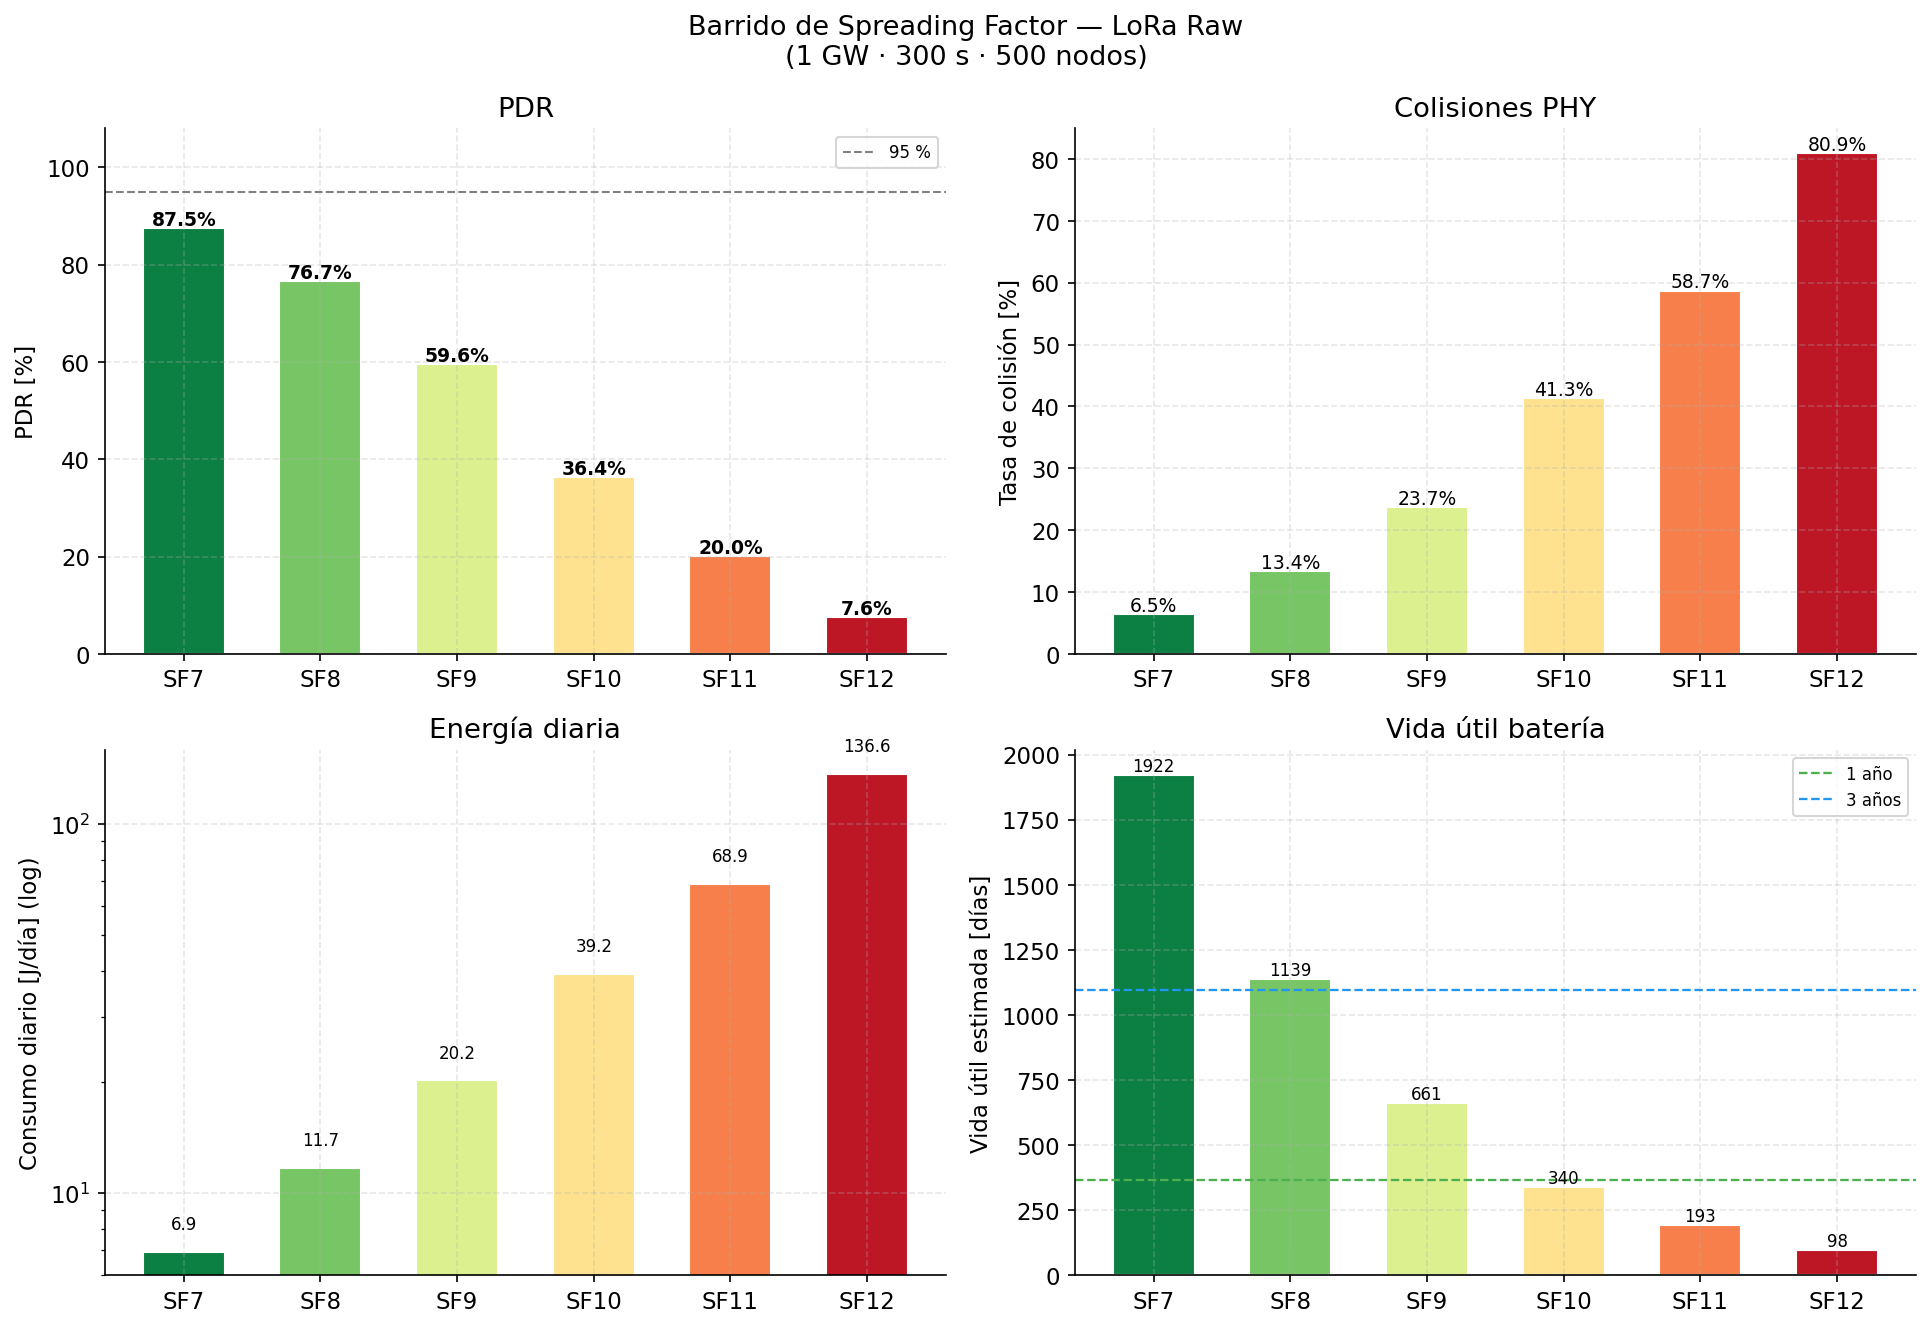
\includegraphics[width=\textwidth]{../graficas/G1_sf_sweep.png}
  \caption{Efecto del SF sobre PDR, colisiones, consumo diario (escala log)
    y vida útil de la batería. Cada incremento en SF dobla el airtime,
    saturando el canal y multiplicando el consumo energético.}
  \label{fig:sf_sweep}
\end{figure}

\textbf{Análisis:} El SF es el parámetro de mayor impacto en la red.
La tasa de colisión crece de 6.5\,\% (SF7) a 80.9\,\% (SF12), colapsando
el PDR. Simultáneamente, el consumo aumenta $19.7\times$ (de 6.93 a
136.6\,J/día), reduciendo la vida útil de 5.3 años a 98 días.
\textbf{SF7 es el único SF viable} para redes densas de LoRa raw:
ofrece el mejor balance entre enlace (sensibilidad $-123$\,dBm) y
capacidad de canal.

\subsection{Barrido de intervalo de transmisión}

\begin{table}[H]
\centering
\caption{Efecto del intervalo heartbeat (SF7, 1 GW, 500 nodos).}
\label{tab:hb_sweep}
\begin{tabular}{rrrrrr}
\toprule
\textbf{Intervalo} & \textbf{Paquetes/h} & \textbf{PDR} &
  \textbf{Colisión} & \textbf{J/día} & \textbf{Vida útil} \\
\midrule
   60\,s & 30\,428 & 48.1\% & 32.4\% & 28.63 &   465 días \\
  150\,s & 12\,428 & 74.9\% & 14.6\% & 12.36 & 1\,078 días \\
  300\,s &  6\,428 & 87.5\% &  6.5\% &  6.93 & 1\,922 días \\
  600\,s &  3\,428 & 94.0\% &  3.4\% &  4.22 & 3\,157 días \\
1\,200\,s &  1\,928 & 96.2\% &  2.0\% &  2.86 & 4\,654 días \\
\bottomrule
\end{tabular}
\end{table}

\begin{figure}[H]
  \centering
  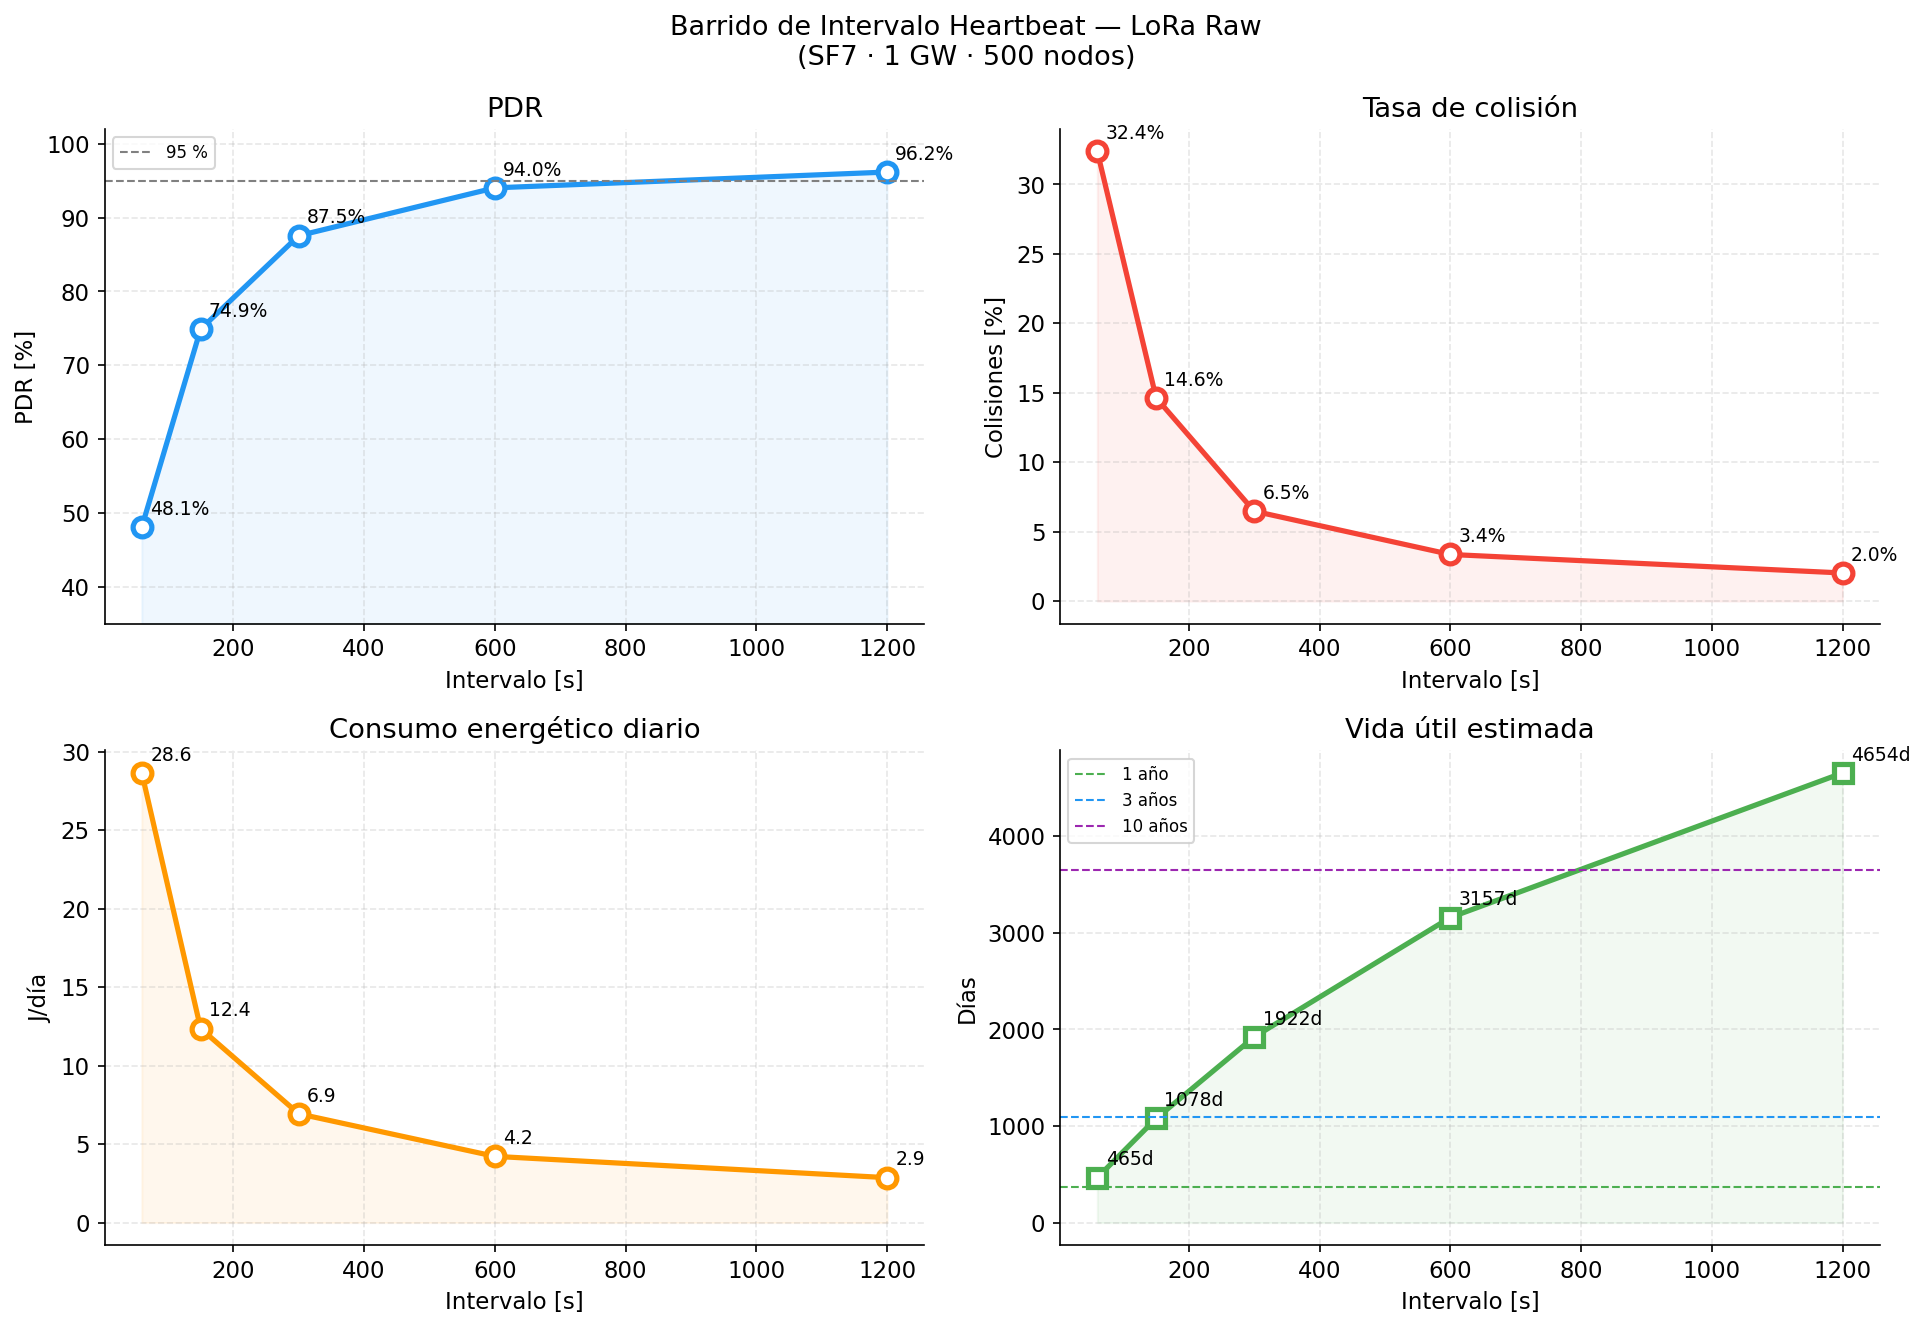
\includegraphics[width=\textwidth]{../graficas/G3_heartbeat_sweep.png}
  \caption{Relación entre intervalo de transmisión, PDR, colisiones,
    consumo diario y vida útil estimada. A mayor intervalo: menor carga
    del canal, mayor PDR y mayor vida útil.}
  \label{fig:hb_sweep}
\end{figure}

\textbf{Análisis:} El intervalo de transmisión tiene un efecto doble:
\begin{enumerate}
  \item \textbf{Energético:} reducir la frecuencia de 60\,s a 1\,200\,s
    baja el consumo $10\times$ (de 28.63 a 2.86\,J/día).
  \item \textbf{Canal:} menor carga reduce colisiones de 32.4\,\% a 2.0\,\%.
\end{enumerate}

El \textbf{intervalo óptimo es 300\,s}: actualización cada 5 minutos,
suficiente para gestión de estacionamiento, con PDR = 87.5\% y vida útil
de 5.3 años. Para aplicaciones que priorizan confiabilidad, 600\,s eleva
el PDR a 94.0\,\% con la mitad del consumo.

\subsection{Energía y modelo solar}

Sin ventanas RX, el modelo de energía diaria se simplifica a:

\begin{equation}
  E_\text{día} = P_\text{TX}\,t_\text{TX} + P_\text{sleep}\,(86\,400 - t_\text{TX})
\end{equation}

Para SF7 y 308 paquetes/día ($= 288$ heartbeat $+ 20$ eventos):

\begin{align}
  t_\text{TX}    &= 308 \times 0.0566\,\text{s} = 17.43\,\text{s/día}
                   \quad (\text{duty cycle} = 0.020\%) \\
  E_\text{TX}    &= (0.090 \times 3.7)\,\text{W} \times 17.43\,\text{s}
                  = 5.80\,\text{J/día} \\
  E_\text{sleep} &= (3.5\times10^{-6} \times 3.7)\,\text{W}
                   \times 86383\,\text{s} = 1.12\,\text{J/día} \\
  \mathbf{E_\text{día}} &= \mathbf{6.92\,\text{J/día}}
  \quad (\text{medido en simulación: } 6.93\,\text{J/día},\; \Delta < 0.1\%)
\end{align}

\begin{equation}
  P_\text{avg} = \frac{6.92}{86\,400} = 80.1\,\mu\text{W}
  \qquad
  t_\text{vida} = \frac{13\,320\,\text{J}}{6.92\,\text{J/día}}
  = \mathbf{1\,924\,\text{días} \approx 5.3\,\text{años}}
\end{equation}

Con el panel solar de 5\,V/55\,mA (275\,mW pico) y $H_\text{sun} = 5.5$\,h/día
(Boulder, CO):

\begin{equation}
  E_\text{cosecha} = 275\,\text{mW} \times 0.166 \times 5.5 \times 3\,600
  = 909\,\text{J/día}
  \gg E_\text{día} = 6.92\,\text{J/día}
  \quad \left(\text{margen: } 131\times\right)
\end{equation}

\begin{figure}[H]
  \centering
  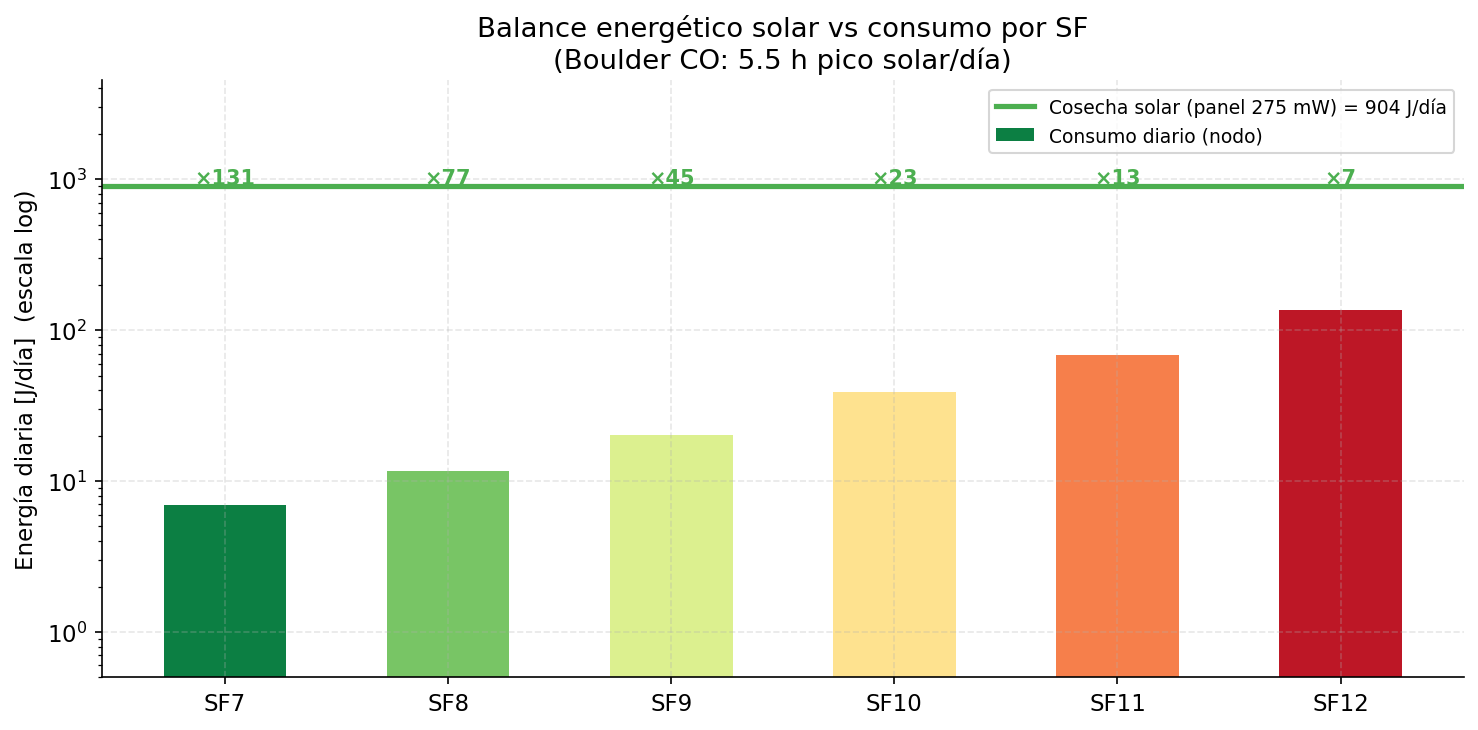
\includegraphics[width=0.9\textwidth]{../graficas/G9_solar_balance.png}
  \caption{Balance energético solar vs.\ consumo por SF (escala log).
    Para SF7–SF9 la cosecha solar supera el consumo por un factor $> 10$.
    Solo SF12 es solar-inviable con un panel pequeño.}
  \label{fig:solar}
\end{figure}

\begin{figure}[H]
  \centering
  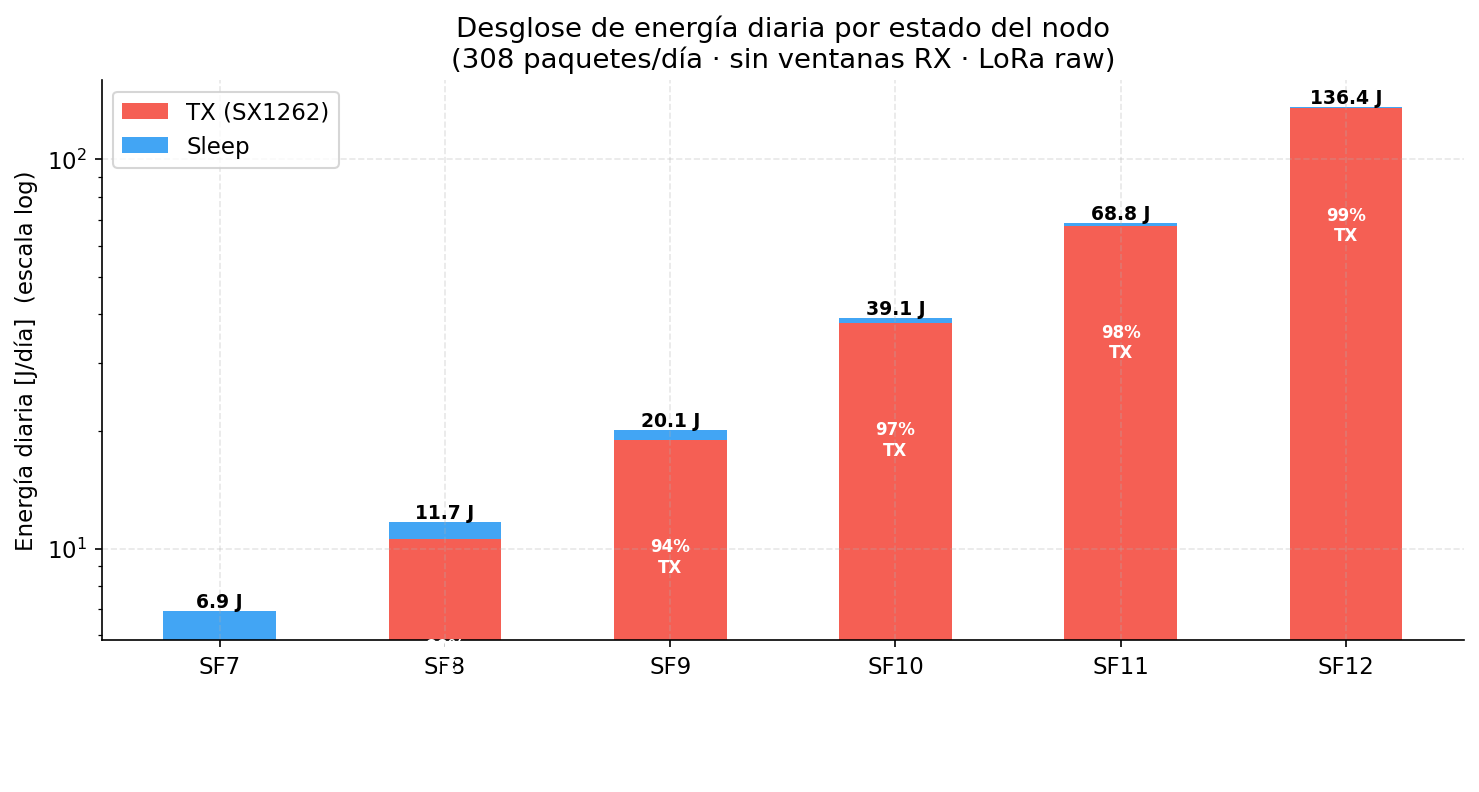
\includegraphics[width=0.85\textwidth]{../graficas/G8_energy_breakdown.png}
  \caption{Desglose analítico de energía diaria por estado del nodo.
    En SF7, el 84\,\% del consumo corresponde a TX y solo el 16\,\% a sleep.
    En SF12 el tiempo en TX es tan elevado que domina completamente.}
  \label{fig:energy_breakdown}
\end{figure}

\begin{figure}[H]
  \centering
  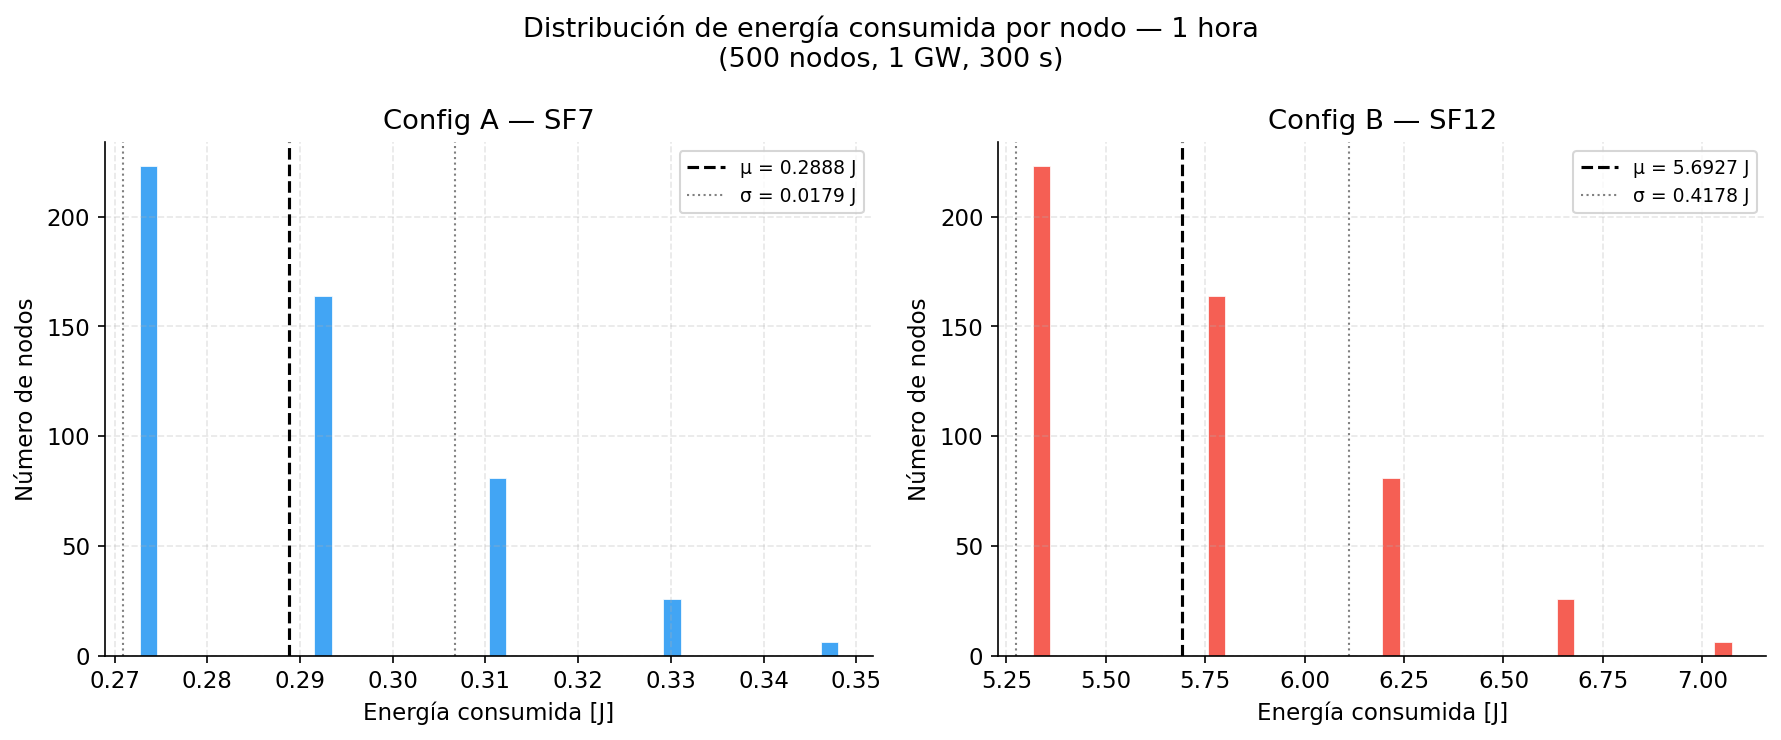
\includegraphics[width=0.9\textwidth]{../graficas/G5_energy_distribution.png}
  \caption{Distribución del consumo por nodo en 1 hora de simulación.
    SF7 ($\sigma = 0.018$\,J, CV = 6.2\,\%) muestra alta uniformidad entre nodos,
    lo que facilita el dimensionamiento homogéneo del sistema.
    SF12 presenta mayor dispersión ($\sigma = 0.417$\,J) por los patrones
    de colisión dependientes de la posición.}
  \label{fig:energy_dist}
\end{figure}

\subsection{Vida útil con degradación de batería LiPo}

La degradación se modela con el modelo \textbf{KWW}
(\emph{Kohlrausch–Williams–Watts}, exponencial estirado):

\begin{equation}
  C(N) = C_0 \cdot \exp\!\left[-\left(\frac{N}{\tau}\right)^{\!\beta}\right],
  \quad \tau = 1\,425\;\text{ciclos},\quad \beta = 1.424
  \label{eq:kww}
\end{equation}

Con $\beta > 1$ la degradación es acelerada al final de la vida
(efecto \emph{knee} en el día $\approx 573$, año 1.6). A diferencia
del modelo lineal, la capacidad nunca llega a cero de forma abrupta.

\begin{figure}[H]
  \centering
  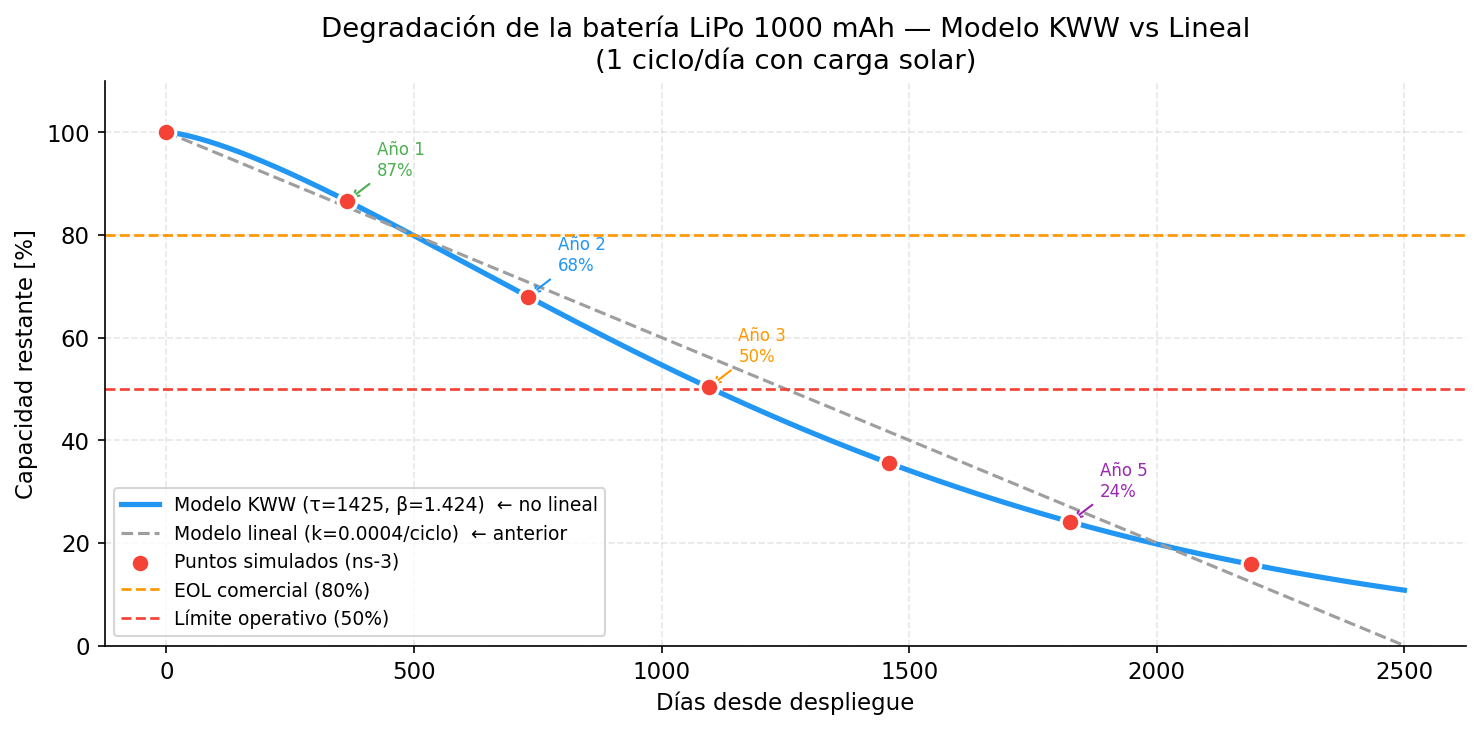
\includegraphics[width=0.9\textwidth]{../graficas/GD1_battery_degradation.png}
  \caption{Curva de degradación KWW vs.\ lineal. Los puntos rojos son
    los 7 escenarios simulados en ns-3. El modelo KWW captura el
    efecto \emph{knee} real de las celdas LiPo.}
  \label{fig:degrade_curve}
\end{figure}

\begin{table}[H]
\centering
\caption{Autonomía sin recarga solar a lo largo de la vida del nodo
  (SF7, 300\,s, modelo KWW).}
\label{tab:degrade}
\begin{tabular}{rrrrl}
\toprule
\textbf{Día} & \textbf{Año} & \textbf{Capacidad} &
  \textbf{Autonomía sin solar} & \textbf{Con solar} \\
\midrule
    0 & 0   & 13\,320\,J (100.0\,\%) & 1\,922 días & $\checkmark$ ($\times131$) \\
  365 & 1   & 11\,536\,J (86.6\,\%)  & 1\,665 días & $\checkmark$ ($\times131$) \\
  730 & 2   &  9\,057\,J (68.0\,\%)  & 1\,307 días & $\checkmark$ ($\times131$) \\
 1095 & 3   &  6\,700\,J (50.3\,\%)  &   967 días  & $\checkmark$ ($\times131$) \\
 1460 & 4   &  4\,731\,J (35.5\,\%)  &   683 días  & $\checkmark$ ($\times131$) \\
 1825 & 5   &  3\,212\,J (24.1\,\%)  &   464 días  & $\checkmark$ ($\times131$) \\
 2190 & 6   &  2\,107\,J (15.8\,\%)  &   304 días  & $\checkmark$ ($\times131$) \\
 2500 & 6.8 &  1\,437\,J (10.8\,\%)  &   207 días  & $\checkmark$ ($\times131$) \\
\bottomrule
\end{tabular}
\end{table}

Con panel solar, el sistema opera energéticamente neutro
\textbf{durante toda la vida útil de la batería}: el margen $131\times$
mantiene la operación incluso en el mes de mínima irradiancia
(diciembre, $E_\text{cosecha,min} = 578$\,J/día $\gg 6.92$\,J/día).

\begin{figure}[H]
  \centering
  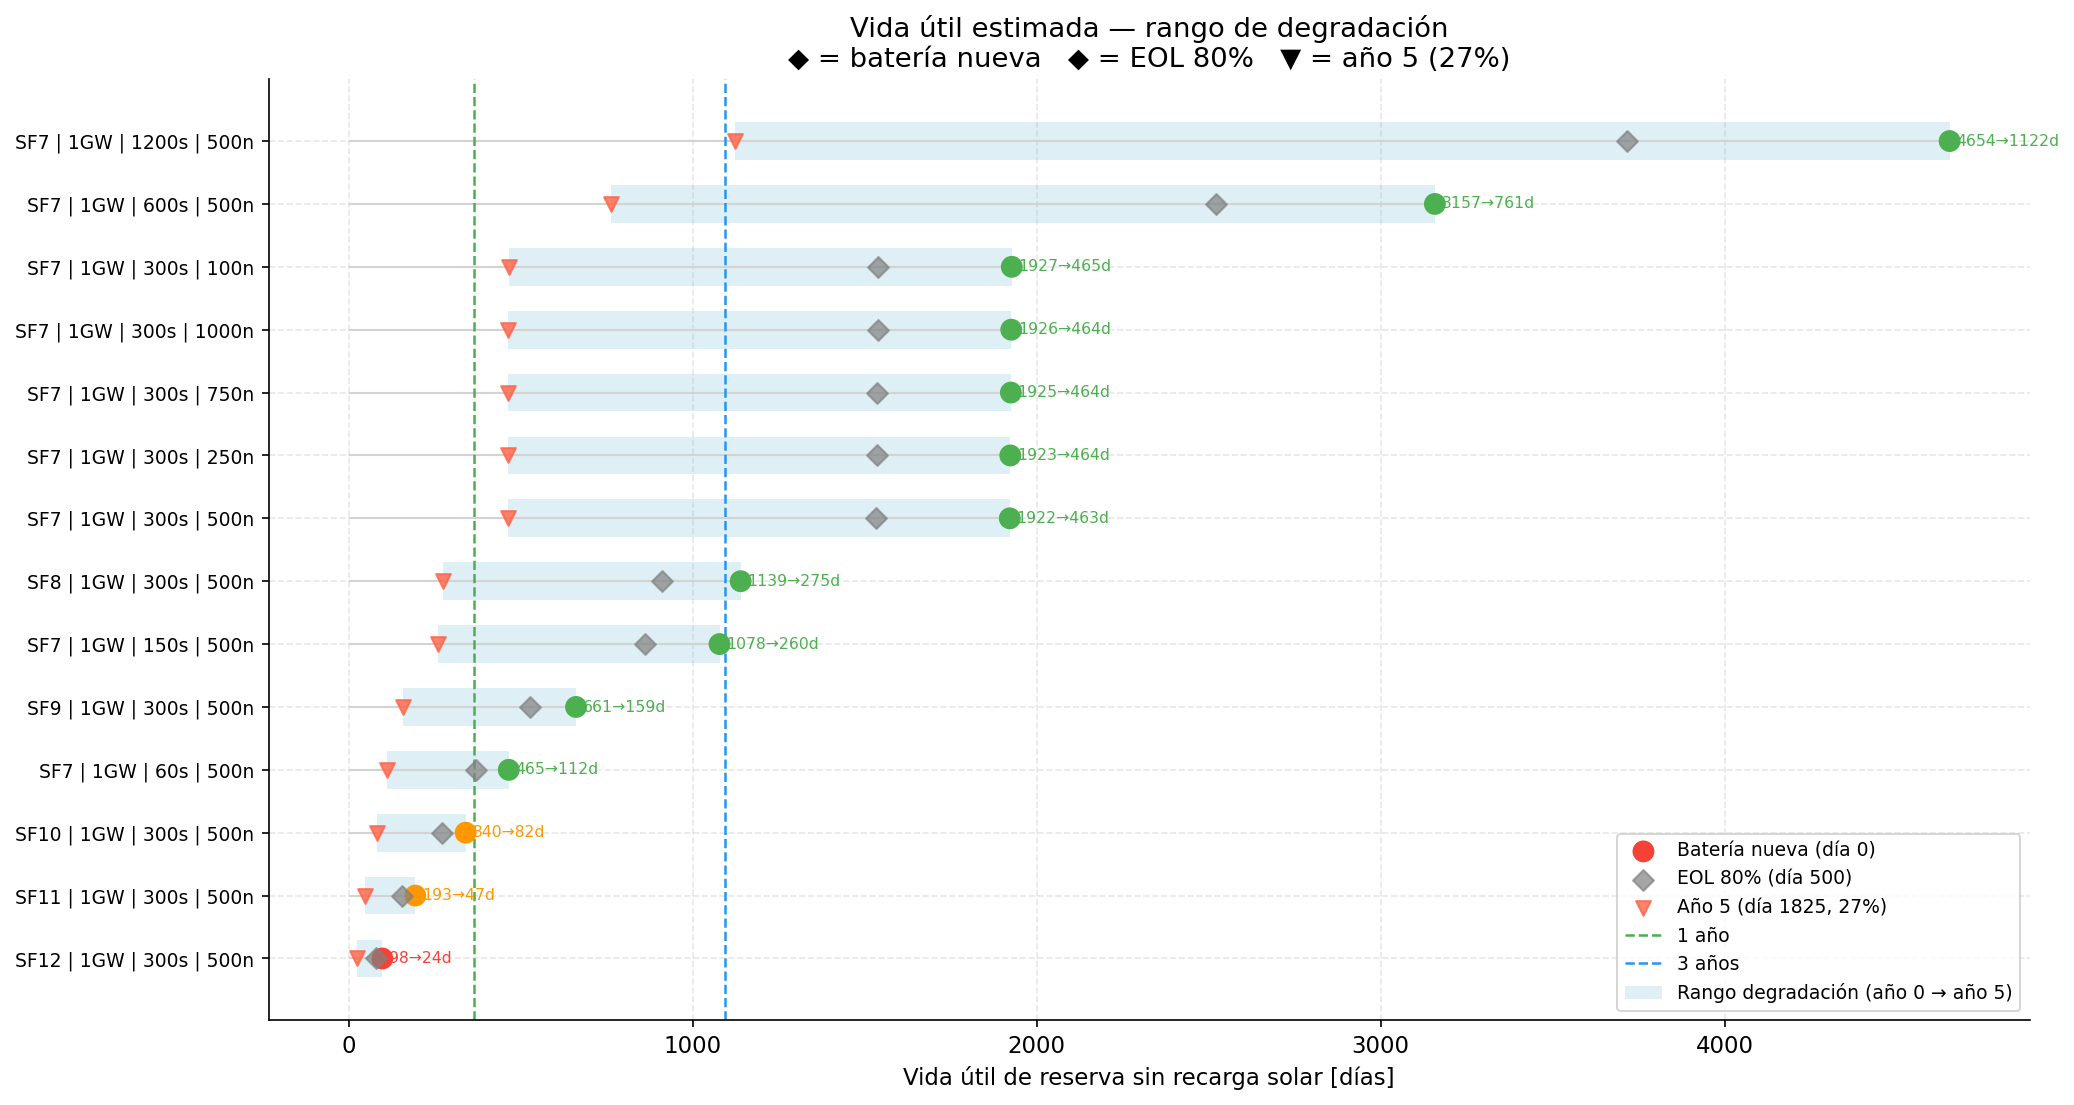
\includegraphics[width=0.85\textwidth]{../graficas/G6_lifetime_all.png}
  \caption{Vida útil estimada para los 14 escenarios: batería nueva (día 0),
    EOL comercial 80\,\% (día 500) y año 5 (día 1\,825). La configuración
    SF7/1\,200\,s supera los 12 años con batería nueva.}
  \label{fig:lifetime_all}
\end{figure}

% ═══════════════════════════════════════════════════════════════════
\section{Análisis de la Escalabilidad}
% ═══════════════════════════════════════════════════════════════════

\begin{table}[H]
\centering
\caption{Escalabilidad: PDR, colisiones y energía vs.\ densidad de nodos
  (SF7, 1 GW, 300\,s heartbeat).}
\label{tab:scalability}
\begin{tabular}{rrrrr}
\toprule
\textbf{Nodos} & \textbf{PDR} & \textbf{Colisión} &
  \textbf{J/nodo/h} & \textbf{Vida útil} \\
\midrule
  100 & 94.8\% &  3.1\% & 0.288 & 1\,927 días \\
  250 & 92.2\% &  4.9\% & 0.289 & 1\,923 días \\
  500 & 87.5\% &  6.5\% & 0.289 & 1\,922 días \\
  750 & 79.2\% & 11.4\% & 0.288 & 1\,925 días \\
1\,000 & 74.5\% & 14.1\% & 0.288 & 1\,926 días \\
\bottomrule
\end{tabular}
\end{table}

\begin{figure}[H]
  \centering
  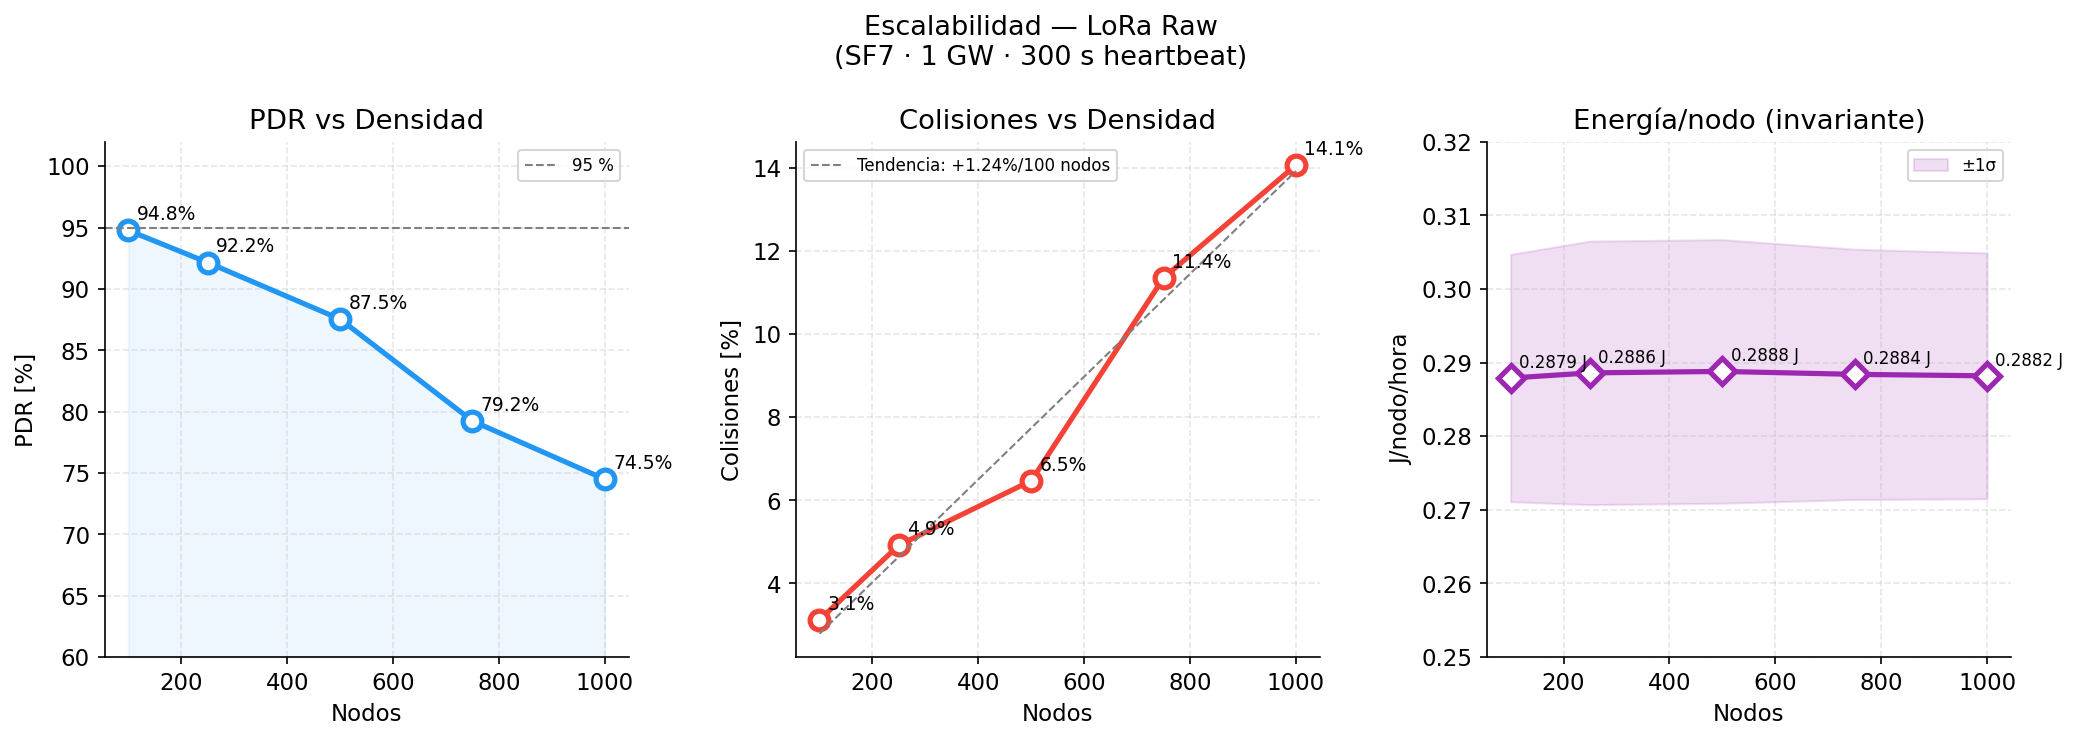
\includegraphics[width=\textwidth]{../graficas/G4_scalability.png}
  \caption{Escalabilidad de la red LoRa raw. PDR y colisión varían
    linealmente con la densidad. La energía por nodo es completamente
    invariante: cada nodo consume lo mismo independientemente de cuántos
    vecinos tenga.}
  \label{fig:scalability}
\end{figure}

\textbf{Observaciones clave:}
\begin{enumerate}
  \item \textbf{Degradación lineal y predecible del PDR:} cada 100 nodos
    adicionales reducen el PDR en $\approx 2.1$ puntos porcentuales y aumentan
    la tasa de colisión en $\approx 1.4$\,pp.
  \item \textbf{Energía invariante respecto a la densidad:} la energía por
    nodo es 0.288--0.289\,J/h en todos los escenarios, confirmando que
    en LoRa raw el consumo depende exclusivamente del comportamiento
    individual del nodo (SF, heartbeat), no de la densidad de la red.
    Esto simplifica el dimensionamiento: todos los nodos son intercambiables.
  \item \textbf{Límite de densidad con 1 GW y SF7:} con 500 nodos el PDR
    = 87.5\,\%, aceptable para conteo vehicular; con 1\,000 nodos cae a
    74.5\,\% — degradación significativa. Para densidades $> 500$ nodos/km²
    se recomienda aumentar el heartbeat a 600\,s (PDR = 94.0\,\%).
  \item \textbf{El cuello de botella es la colisión PHY, no la energía:}
    incluso con 1\,000 nodos el consumo energético individual no varía;
    la limitación es la ocupación del canal compartido.
\end{enumerate}

\begin{figure}[H]
  \centering
  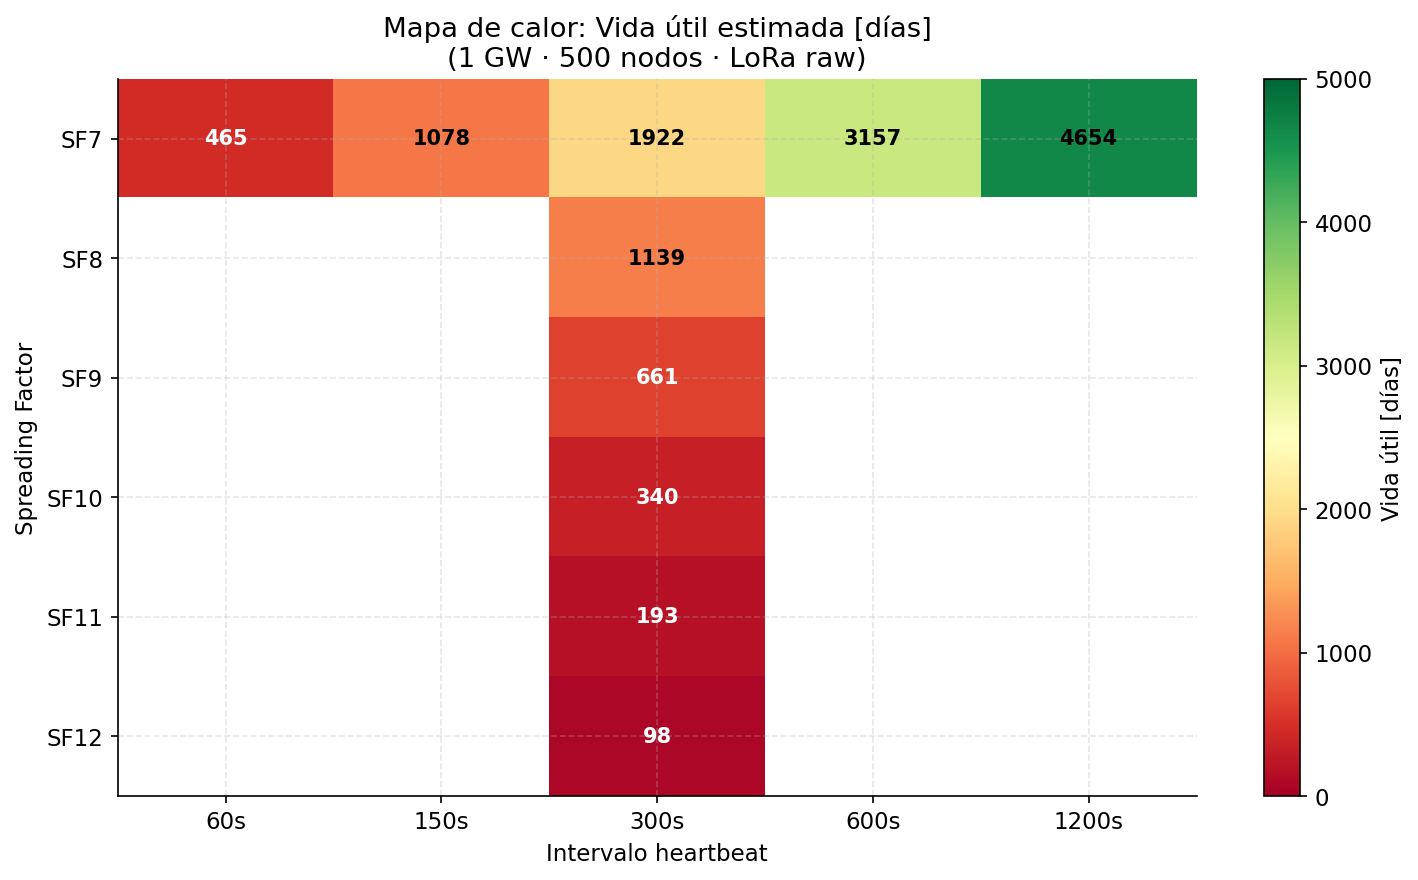
\includegraphics[width=0.85\textwidth]{../graficas/G7_lifetime_heatmap.png}
  \caption{Mapa de calor de vida útil estimada (días) en función del SF y
    el intervalo heartbeat. La región verde (SF7, heartbeat $\geq 600$\,s)
    supera los 3\,000 días. Cualquier combinación con SF $\geq 10$ cae en
    zona roja incluso con heartbeat de 300\,s.}
  \label{fig:heatmap}
\end{figure}

\begin{figure}[H]
  \centering
  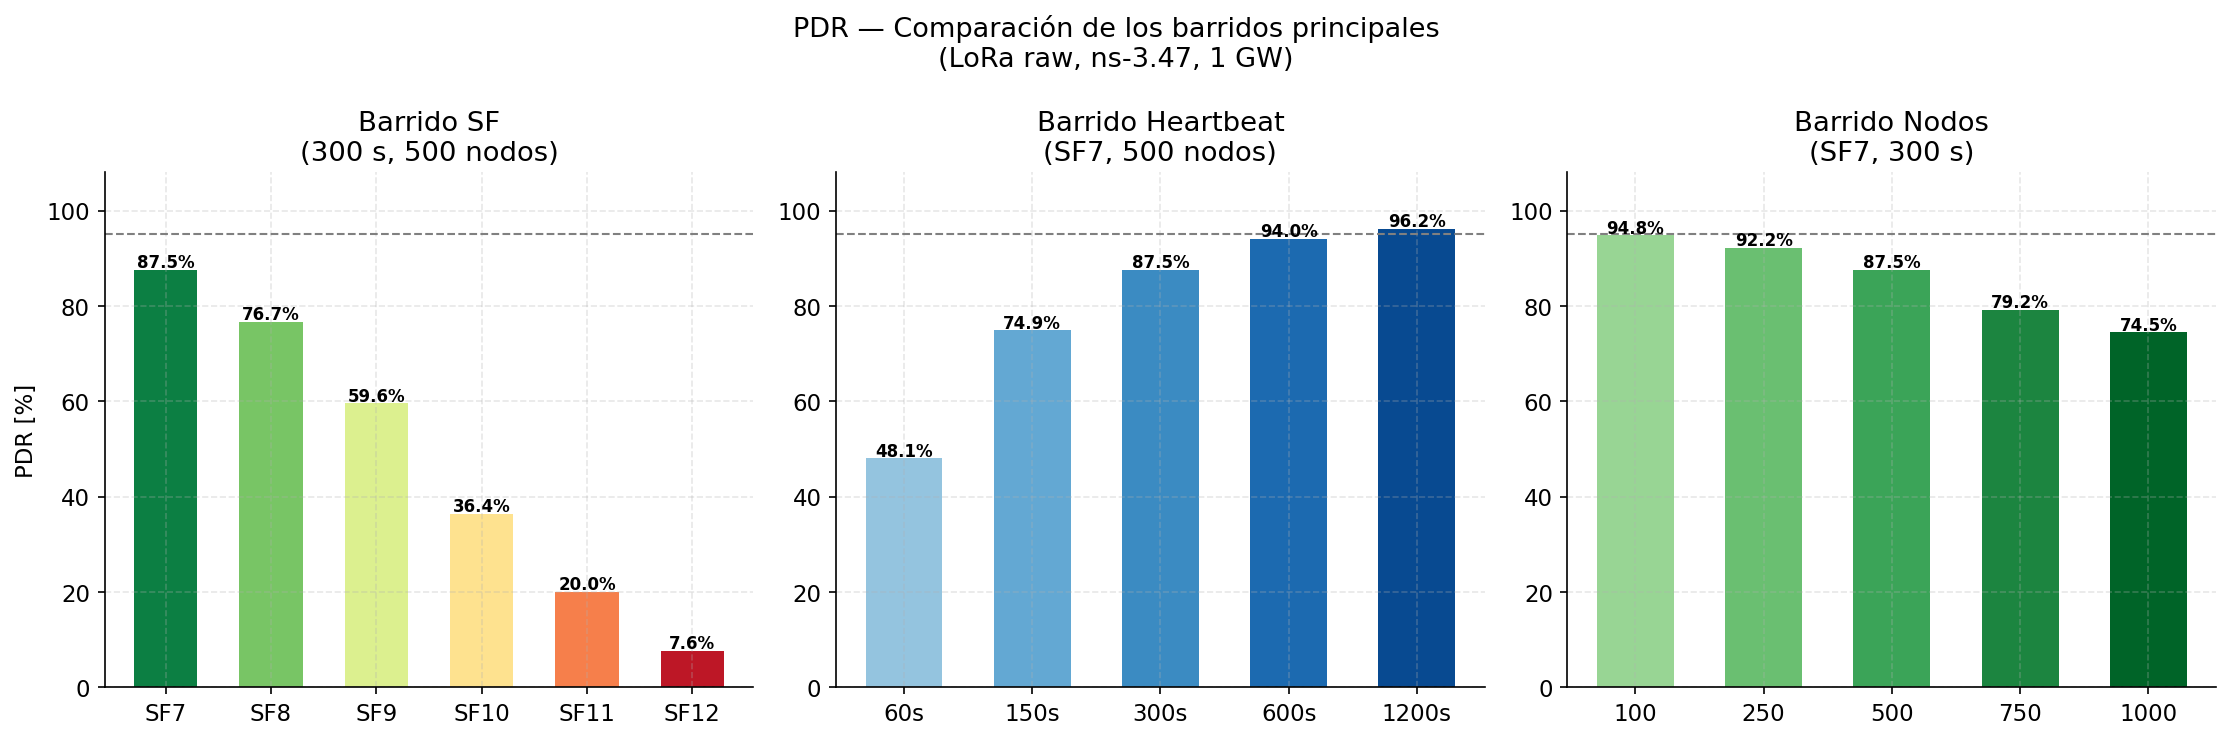
\includegraphics[width=\textwidth]{../graficas/G10_pdr_comparison.png}
  \caption{Comparación de PDR en los tres barridos principales.
    El heartbeat y el SF son los factores de mayor impacto;
    la densidad de nodos tiene un efecto secundario.}
  \label{fig:pdr_comparison}
\end{figure}

\begin{figure}[H]
  \centering
  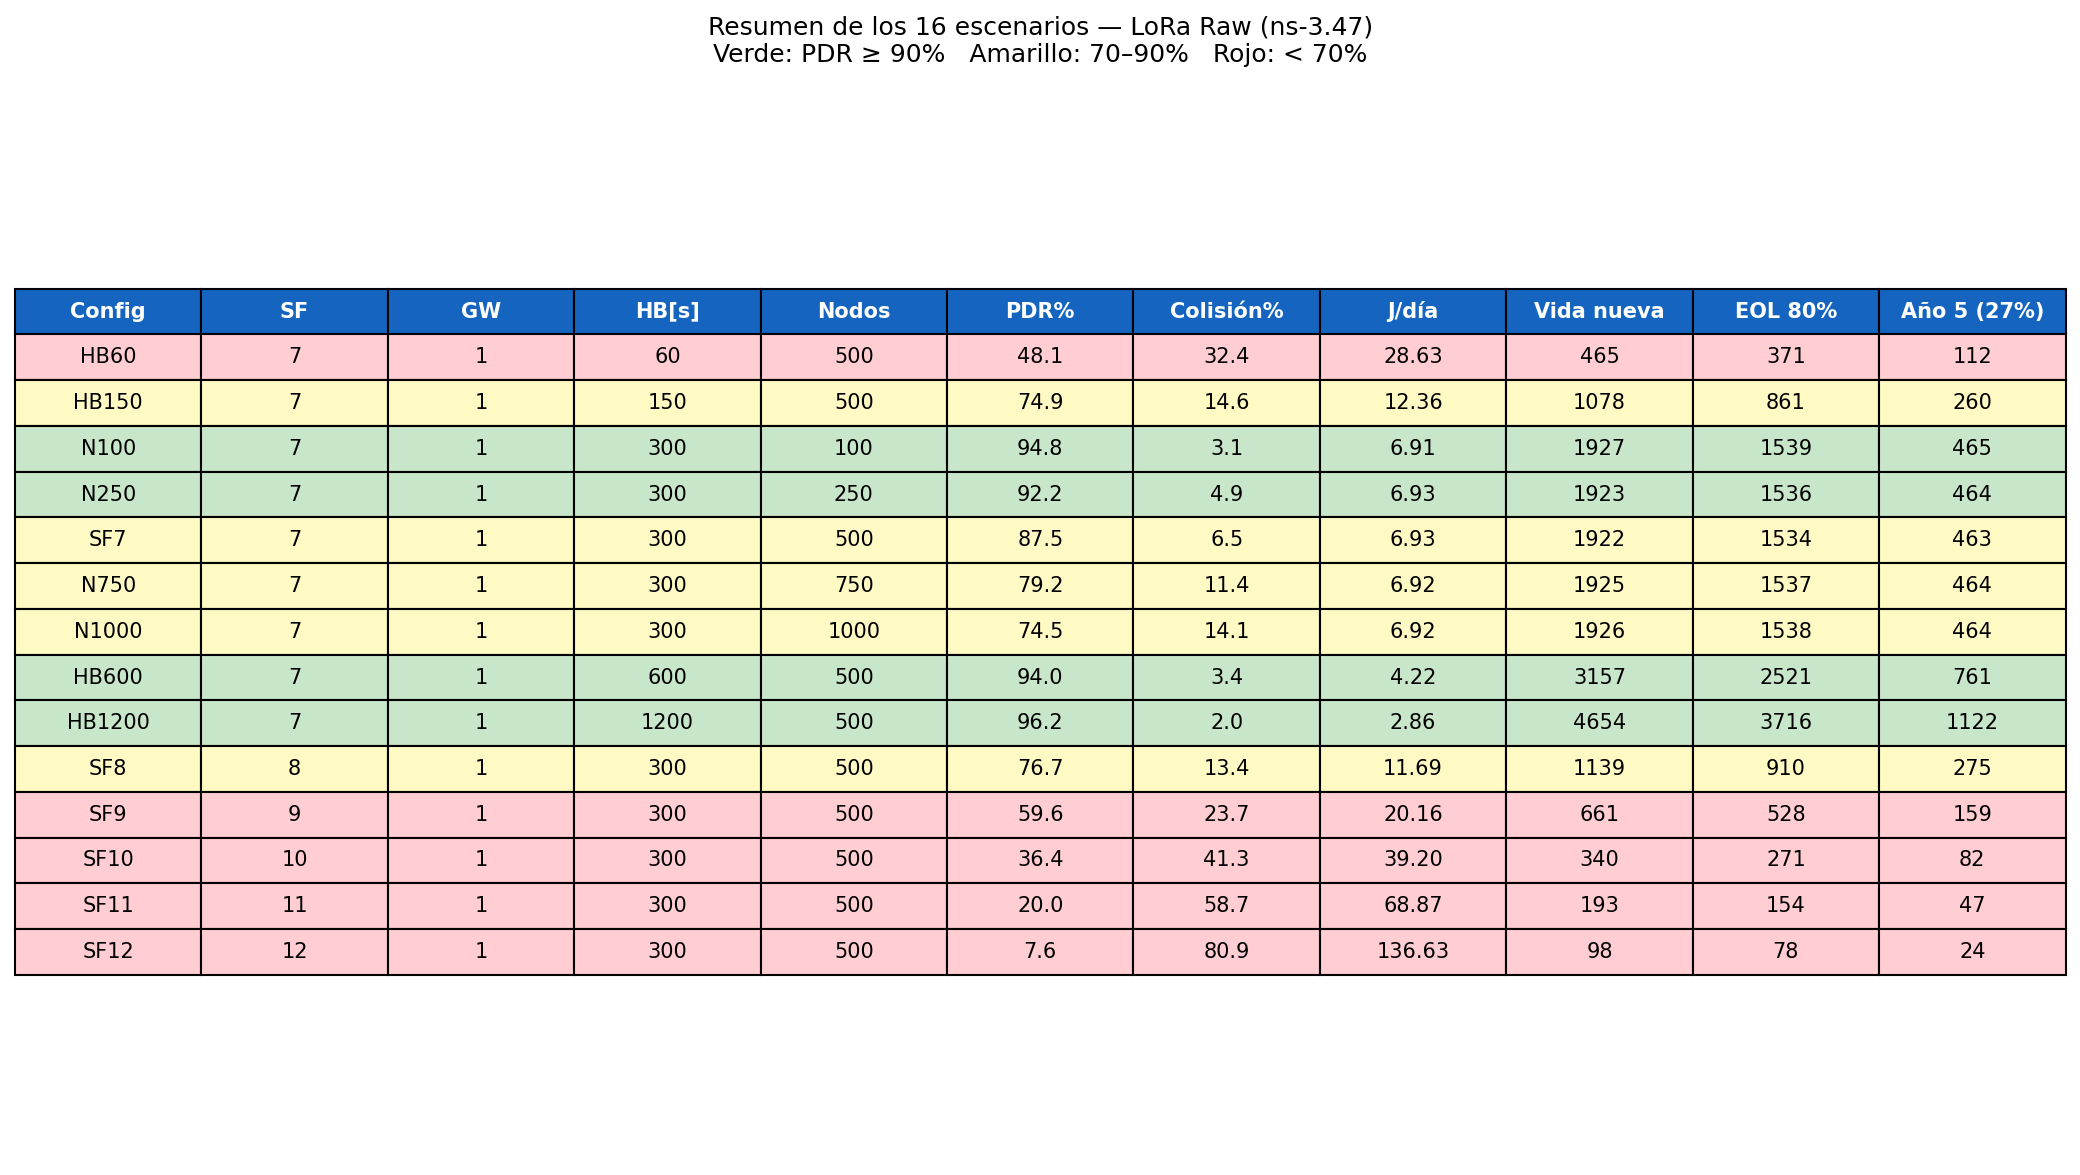
\includegraphics[width=\textwidth]{../graficas/G11_summary_table.png}
  \caption{Tabla resumen visual de los 14 escenarios, coloreados por PDR.
    Verde: PDR $\geq 90$\,\%, Amarillo: 70--90\,\%, Rojo: $<70$\,\%.}
  \label{fig:summary_table}
\end{figure}

% ═══════════════════════════════════════════════════════════════════
\section{Estimación de Costos Energéticos}
% ═══════════════════════════════════════════════════════════════════

\subsection{Energía por paquete transmitido}

La energía consumida en una sola transmisión depende del SF a través del
airtime:

\begin{equation}
  E_\text{TX/pkt}(SF) = I_\text{TX} \times V_\text{bat} \times T_\text{air}(SF)
  = 0.090\,\text{A} \times 3.7\,\text{V} \times T_\text{air}(SF)
\end{equation}

\begin{table}[H]
\centering
\caption{Costo energético por paquete transmitido y por paquete
  \emph{entregado exitosamente} (500 nodos, 1 GW, 300\,s heartbeat).}
\label{tab:energy_per_pkt}
\begin{tabular}{rrrrr}
\toprule
\textbf{SF} & \textbf{$T_\text{air}$} & \textbf{$E_\text{TX/pkt}$} &
  \textbf{PDR} & \textbf{$E_\text{TX/pkt exitoso}$} \\
\midrule
 7 &    56.6\,ms &  18.9\,mJ &  87.5\% &  21.6\,mJ \\
 8 &   103.7\,ms &  34.5\,mJ &  76.7\% &  45.0\,mJ \\
 9 &   205.8\,ms &  68.5\,mJ &  59.6\% & 114.9\,mJ \\
10 &   411.6\,ms & 137.0\,mJ &  36.4\% & 376.4\,mJ \\
11 &   823.3\,ms & 274.2\,mJ &  20.0\% & 1\,371\,mJ \\
12 & 1\,318.9\,ms & 439.3\,mJ &   7.6\% & 5\,780\,mJ \\
\bottomrule
\end{tabular}
\end{table}

La energía por paquete exitoso de SF12 es \textbf{268$\times$ mayor} que
la de SF7, combinando el mayor airtime con el altísimo desperdicio por
colisiones. El costo energético real de una transmisión exitosa es la
métrica relevante para el diseño del sistema.

\subsection{Eficiencia energética: J por bit entregado}

\begin{equation}
  \eta(SF) = \frac{E_\text{TX/pkt exitoso}}{N_\text{bits/pkt}}
           = \frac{E_\text{TX/pkt}}{PDR(SF) \times 160\,\text{bits}}
\end{equation}

\begin{table}[H]
\centering
\caption{Eficiencia energética por bit entregado exitosamente.}
\label{tab:energy_per_bit}
\begin{tabular}{rrrr}
\toprule
\textbf{SF} & \textbf{PDR} & \textbf{$E$/bit exitoso} &
  \textbf{Factor vs SF7} \\
\midrule
 7 &  87.5\% &  134.6\,$\mu$J/bit & $1.0\times$ \\
 8 &  76.7\% &  281.3\,$\mu$J/bit & $2.1\times$ \\
 9 &  59.6\% &  718.6\,$\mu$J/bit & $5.3\times$ \\
10 &  36.4\% & 2\,352\,$\mu$J/bit & $17.5\times$ \\
11 &  20.0\% & 8\,569\,$\mu$J/bit & $63.6\times$ \\
12 &   7.6\% & 36\,131\,$\mu$J/bit & $268.5\times$ \\
\bottomrule
\end{tabular}
\end{table}

SF7 es \textbf{268$\times$ más eficiente} en términos de J/bit entregado
que SF12. El aumento del SF degrada la eficiencia tanto por mayor airtime
como por mayor tasa de colisiones, haciendo que la energía invertida en
transmisiones fallidas sea desperdiciada.

\subsection{Energía desperdiciada por colisiones}

En LoRa raw no existe ARQ (retransmisión automática), por lo que la
energía de los paquetes colisionados se pierde irrecuperablemente.
El desperdicio diario por colisiones en cada nodo es:

\begin{equation}
  E_\text{desperdicio}(SF) = N_\text{pkts/día} \times P_\text{colisión}(SF)
    \times E_\text{TX/pkt}(SF)
\end{equation}

\begin{table}[H]
\centering
\caption{Energía diaria desperdiciada por colisiones por nodo
  (500 nodos, 1 GW, 300\,s heartbeat, 308 paquetes/día).}
\label{tab:wasted_energy}
\begin{tabular}{rrrrrr}
\toprule
\textbf{SF} & \textbf{Colisión} & \textbf{Pkts perdidos/día} &
  \textbf{$E_\text{TX/pkt}$} & \textbf{$E_\text{desperdicio}$/día} &
  \textbf{\% del total} \\
\midrule
 7 &  6.5\% &  20.0 &  18.9\,mJ &   0.38\,J &  5.5\% \\
 8 & 13.4\% &  41.3 &  34.5\,mJ &   1.42\,J & 12.2\% \\
 9 & 23.7\% &  73.0 &  68.5\,mJ &   5.00\,J & 24.8\% \\
10 & 41.3\% & 127.2 & 137.0\,mJ &  17.43\,J & 44.5\% \\
11 & 58.7\% & 180.8 & 274.2\,mJ &  49.57\,J & 72.0\% \\
12 & 80.9\% & 249.2 & 439.3\,mJ & 109.44\,J & 80.1\% \\
\bottomrule
\end{tabular}
\end{table}

Con SF12, el 80.1\,\% de la energía de transmisión diaria se desperdicia
en colisiones. Con SF7 el desperdicio es solo del 5.5\,\%
(0.38\,J/día/nodo), aceptable en el contexto del presupuesto energético
total de 6.93\,J/día.

\subsection{Presupuesto energético diario por nodo}

\begin{table}[H]
\centering
\caption{Desglose del presupuesto energético diario por nodo (SF7,
  300\,s heartbeat). Valores calculados analíticamente y verificados
  en simulación.}
\label{tab:energy_budget}
\begin{tabular}{lrrr}
\toprule
\textbf{Estado} & \textbf{Tiempo/día} & \textbf{Potencia} & \textbf{Energía/día} \\
\midrule
Transmisión (TX)    & 17.43\,s    & 333\,mW  & 5.80\,J  \\
Sleep               & 86\,383\,s  & 12.95\,$\mu$W & 1.12\,J \\
\midrule
\textbf{Total consumo}  & 86\,400\,s & 80.1\,$\mu$W & \textbf{6.92\,J} \\
\midrule
Cosecha solar       & 5.5\,h pico &  275\,mW ($\eta=16.6$\%) & 909\,J \\
\textbf{Balance neto}   & —       & —         & \textbf{+902\,J/día} \\
\bottomrule
\end{tabular}
\end{table}

\begin{figure}[H]
  \centering
  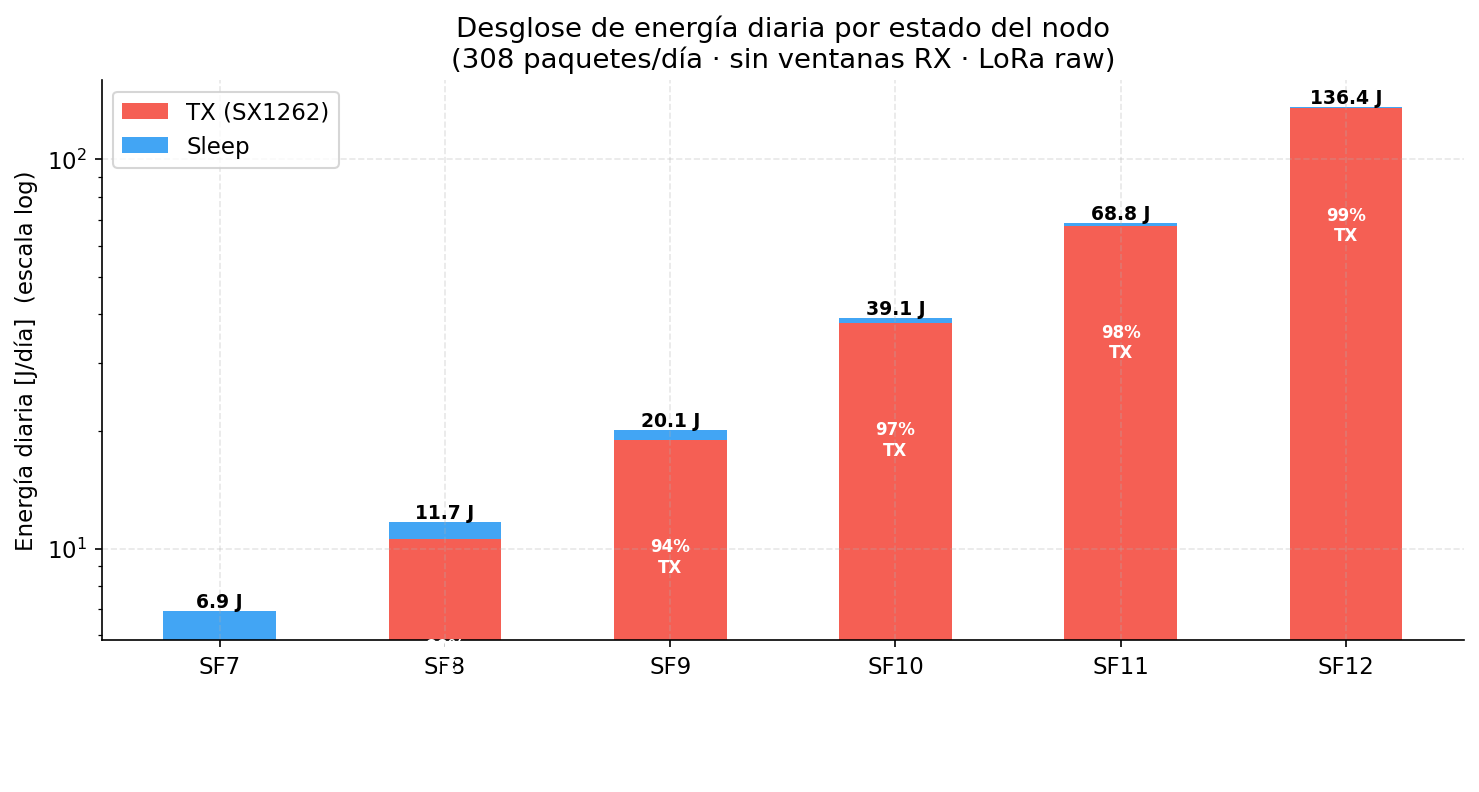
\includegraphics[width=0.9\textwidth]{../graficas/G8_energy_breakdown.png}
  \caption{Desglose analítico de energía diaria por SF. En SF7 la
    transmisión representa el 84\,\% del consumo total; en SF12 domina
    completamente ($>$99.9\,\%).}
  \label{fig:energy_budget}
\end{figure}

\subsection{Consumo energético total de la red}

Con 500 nodos y SF7/300\,s, el consumo energético agregado de la red es:

\begin{align}
  E_\text{red/día}  &= 500 \times 6.92\,\text{J} = 3\,460\,\text{J/día}
                      = 0.961\,\text{Wh/día} \\
  E_\text{red/año}  &= 500 \times 6.92 \times 365 = 1\,262\,900\,\text{J/año}
                      = 350.8\,\text{Wh/año} \\
  E_\text{cosecha/día} &= 500 \times 909\,\text{J} = 454\,500\,\text{J/día}
\end{align}

La cosecha solar de la red supera el consumo total en un factor de
$131\times$, lo que garantiza operación energéticamente neutra incluso
asumiendo solo el 0.76\,\% de eficiencia de conversión solar efectiva.

\subsection{Impacto del heartbeat en el presupuesto energético}

\begin{table}[H]
\centering
\caption{Presupuesto energético por nodo según intervalo heartbeat
  (SF7, 500 nodos). La energía de sleep permanece prácticamente constante
  porque el duty cycle TX nunca supera el 0.2\,\%.}
\label{tab:energy_heartbeat}
\begin{tabular}{rrrrrr}
\toprule
\textbf{Heartbeat} & \textbf{Pkts/día} & \textbf{$E_\text{TX}$/día} &
  \textbf{$E_\text{sleep}$/día} & \textbf{Total} & \textbf{Ratio solar} \\
\midrule
   60\,s & 1\,440 + 20 & 27.50\,J & 1.12\,J & 28.62\,J & $\times$31.8 \\
  150\,s &   576 + 20  & 11.22\,J & 1.12\,J & 12.34\,J & $\times$73.7 \\
  300\,s &   288 + 20  &  5.80\,J & 1.12\,J &  6.92\,J & $\times$131 \\
  600\,s &   144 + 20  &  3.08\,J & 1.12\,J &  4.20\,J & $\times$216 \\
1\,200\,s &  72 + 20  &  1.73\,J & 1.12\,J &  2.85\,J & $\times$319 \\
\bottomrule
\end{tabular}
\end{table}

\textbf{Observación:} incluso con heartbeat de 60\,s (caso más agresivo),
el panel solar produce $31.8\times$ más energía que la consumida
diariamente. El \textbf{piso energético} del sistema está dominado por
el consumo en sleep (1.12\,J/día), que es independiente de la tasa de
transmisión. Aumentar el heartbeat más allá de 1\,200\,s produce
rendimientos decrecientes: el ahorro adicional de TX se vuelve marginal
frente al consumo fijo de sleep.

\end{document}
